\documentclass{simcenterdocumentation}
\usepackage[backend=biber]{biblatex}
\usepackage{subfig}
\usepackage{multirow}
\usepackage{adjustbox} % to adjust table width
\usepackage{graphicx} %Loading the package
\usepackage{longtable}
\usepackage{cleveref}
\graphicspath{{../Common/}{.}} %Setting the graphicspath
\makeatletter % Search additional directories for inputs
\def\input@path{{../Common/}{.}}
%or: \def\input@path{{/path/to/folder/}{/path/to/other/folder/}}
\makeatother

%% Add unicode support for special characters
%%\usepackage[utf8x]{inputenc}

% To compile this file, run "latex/pdflatex codedoc", then "biber codedoc"b
% (or "bibtex codedoc", if the output from latex asks for that instead),
% and then "latex/pdflatex codedoc" (without the quotes in each case).

% Double spacing, if you want it.  Do not use for the final copy. Can also specify
% draft as a document class option. This will generate double spacing and placeholders
% for title page and header images
%% \def\dsp{\def\baselinestretch{2.0}\large\normalsize}
%% \dsp

\bibliography{../Common/references}

\begin{document}
% Declarations for Front Matter
% Software title followed by optional second line
\title{\textit{s$^3$hark}\\ A Research Tool for Studying the Site Specific Response to Earthquakes}
% Use superscripts to indicate author affiliations
\author{Chaofeng Wang, Pedro Arduino and Frank McKenna}
\institutions{NHERI SimCenter, UC Berkeley}
\softwarename{\textit{s$^3$hark}}
\softwareversion{1.1}
\softwarepage{https://github.com/NHERI-SimCenter/s3hark}

%%% DON'T MESS WITH THESE SETTINGS %%%%%%%%%%%%%%%%%%%%%%%%%%%%%%%%
\hypersetup{pageanchor=false}
\maketitle
\copyrightpage
\acknowledgments

\hypersetup{pageanchor=true}
\begin{frontmatter}

\pagestyle{plain}
{
  \renewcommand{\thispagestyle}[1]{}
  \tableofcontents
  \clearpage
  \listoffigures
  \clearpage
  \listoftables
}

\end{frontmatter}
\pagestyle{somewhatsimple}
%%%%%%%%%%%%%%%%%%%%%%%%%%%%%%%%%%%%%%%%%%%%%%%%%%%%%%%%%%%%%%%%%%%
% Create separate tex files for each chapter and provide them as inputs

\chapter{About}
\label{chap:about}
The intended audience for the \texttt{\getsoftwarename{}} Application (\texttt{\getsoftwarename{}} App) is researchers and practitioners
interested in performing site-specific analysis of soil in  response to earthquakes. \texttt{\getsoftwarename{}}  is the acronym of site-specific seismic hazard analysis and research kit.  \\

This is an open-source research application. The source code at
the \href{https://github.com/NHERI-SimCenter/s3hark}{\texttt{\getsoftwarename{}}
Github page} provides an application that can be used to analyze the response of soil to earthquake scenarios.
The application focuses on simulating wave propagation along soil depth using finite element (FE) method. 

Given that the properties of the soil layers and the earthquake events are known,
 \texttt{\getsoftwarename{}} provides multiple nonlinear material models for simulating the soil behavior under earthquake loading.



This is Version \getsoftwareversion{} of the tool. Users are
encouraged to comment on what additional features and capabilities
they would like to see in this application. These requests and
feedback can be submitted through an anonymous \insertsurveylink{user
survey}; we greatly appreciate any input you have. If there are
features you want, chances are many of your colleagues also would
benefit from them. 


\chapter{Installation Instructions}
\label{chap:installation}
All SimCenter applications are available at
the \href{https://simcenter.designsafe-ci.org/research-tools/overview/}{SimCenter
website} under \emph{Research Tools}. The following sections outline
the steps necessary to download and install the \texttt{\getsoftwarename{}}
application. The SimCenter applications do require that you install a
number of other applications that are needed to run the workflows on
your local machine as well as at DesignSafe. \\


%===============================================================================
\section{Download the Application}
%===============================================================================

% \subsection{Download the Application Files}

To download the \texttt{\getsoftwarename{}} application navigate to
the \getsoftwarepage{\texttt{\getsoftwarename{}} page} and click on
the \emph{Download App \& User Manual} link on the right side of the
page. This will bring you to another page which contains a list of downloadable files and directories.


There are at least four files available for download from this page: 
\begin{enumerate}
    \item The PDF file is the User Manual that you are reading now.
    \item The MOV file is an video that provides an introduction to the usage of the application.
    \item The ZIP file is an archive that contains the application files for a Windows operating system.
    \item The DMG file is an archive that contains the application files for a Mac OS X operating system.
\end{enumerate}

To download the \texttt{\getsoftwarename{}} application click on the link for
the appropriate file for your operating system and then click on the
Download button at bottom right corner of the ensuing pop-up window to
download it. You need to unpackage the application from the downloaded
file and place it in a location on your filesystem. On Windows, we
recommend that you create a \texttt{C:/SimCenter/\getsoftwarename{}}
directory and extract the contents of the \texttt{ZIP} archive
there. It is also recommended to run the included installer for Visual C/C++ runtime library(vc\_redist.x64.exe). On Mac, we recommend you copy the application to either your
Documents folder or your Desktop folder. You are free to place the
applications anywhere you wish, you will just need to make the
appropriate adjustments with the following instructions if you do so. \\



%===============================================================================
\clearpage
\section{Test the \texttt{\getsoftwarename{}} application}
\label{sec:test_local}


Click on the  icon of  \texttt{\getsoftwarename{}} to open the application.
Click the "+" button to add a soil layer (\Cref{fig:addLayer}). Click several times to add more layers.

\begin{figure}[!htbp]
  \centering {
    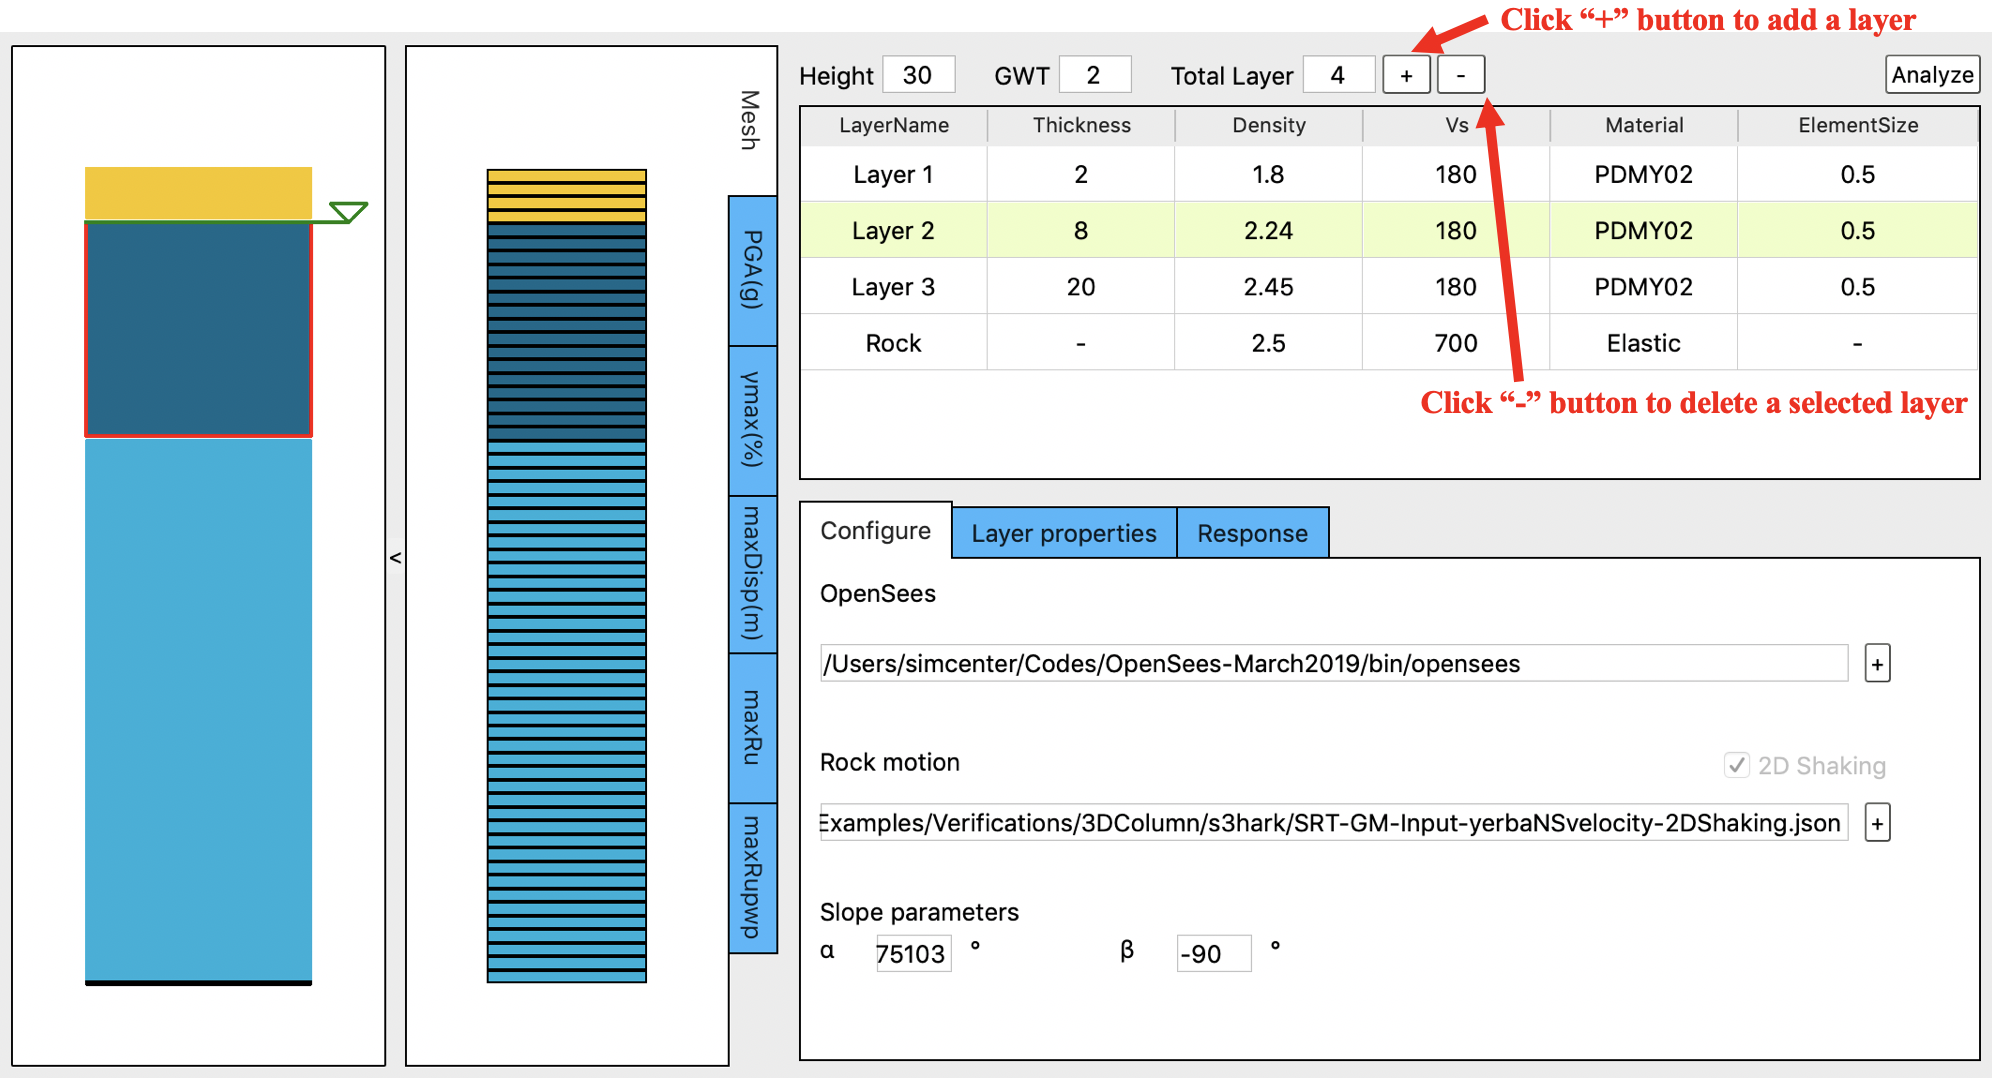
\includegraphics[width=0.9\textwidth]
    {installation/figures/addLayer.png} }
  \caption{Adding soil layers}
  \label{fig:addLayer}
\end{figure}


Click on the configure tab to show configurations options. 
Under the "OpenSees" label, type the path of OpenSees executable. 
You can also select the executable from your local computer by clicking on the "+" button on the right of the input area (\Cref{fig:addOpenSees}).

Under the "Rock motion" label, type the path of a ground motion file. 
You can also select the file from your local computer by clicking on the "+" button on the right of the input area (\Cref{fig:addOpenSees}).

\begin{figure}[!htbp]
  \centering {
    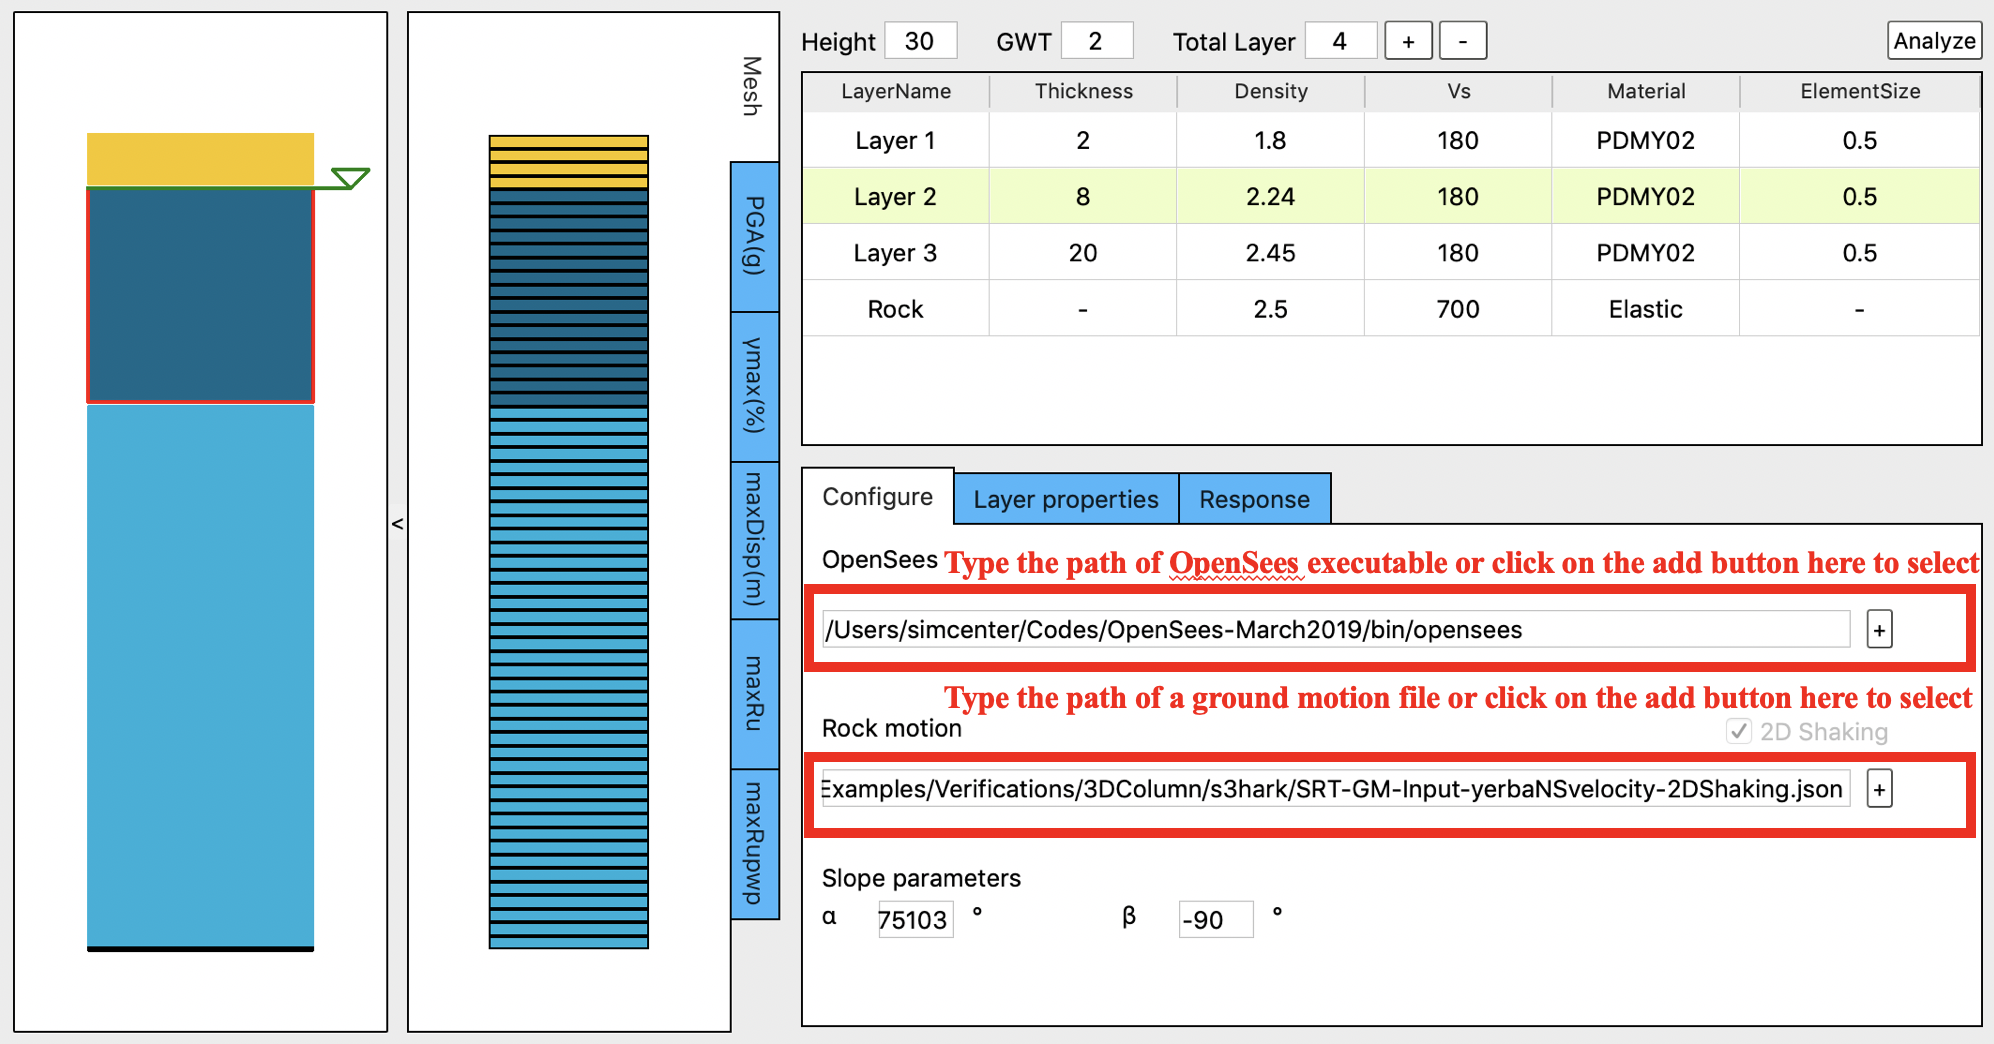
\includegraphics[width=0.9\textwidth]
    {installation/figures/addOpenSees.png} }
  \caption{Adding OpenSees path and rock motion file}
  \label{fig:addOpenSees}
\end{figure}


\begin{figure}[!htbp]
  \centering {
    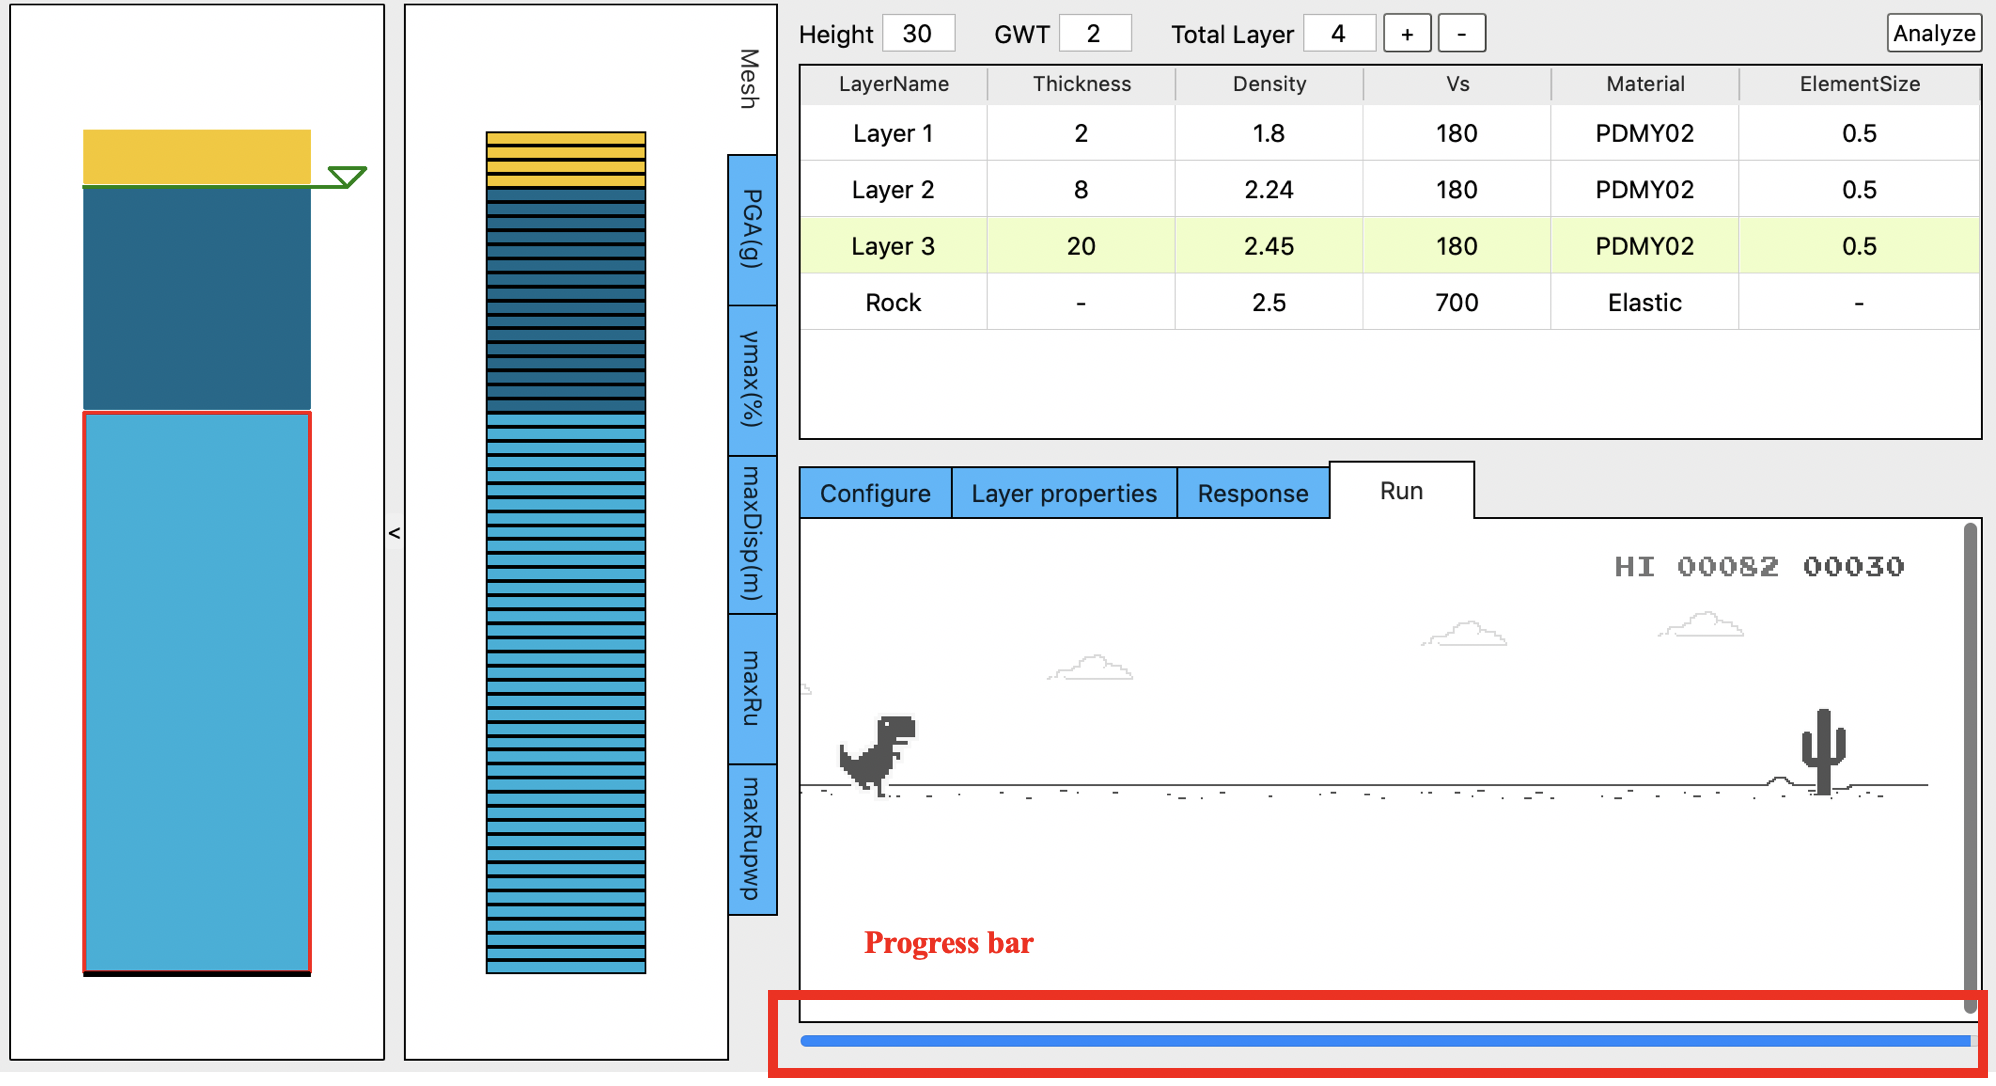
\includegraphics[width=0.9\textwidth]
    {installation/figures/progress.png} }
  \caption{Simulation progress }
  \label{fig:progress}
\end{figure}

Click on the "Analyze" button to run the finite element analysis.
If the soil layers are added successfully, OpenSees path is correct and the rock motion file is correct,
you will see a progress bar (\Cref{fig:prpgress}) displayed at the bottom of the right hand side of the app, which shows the percentage of steps performed. 

\begin{figure}[!htbp]
  \centering {
    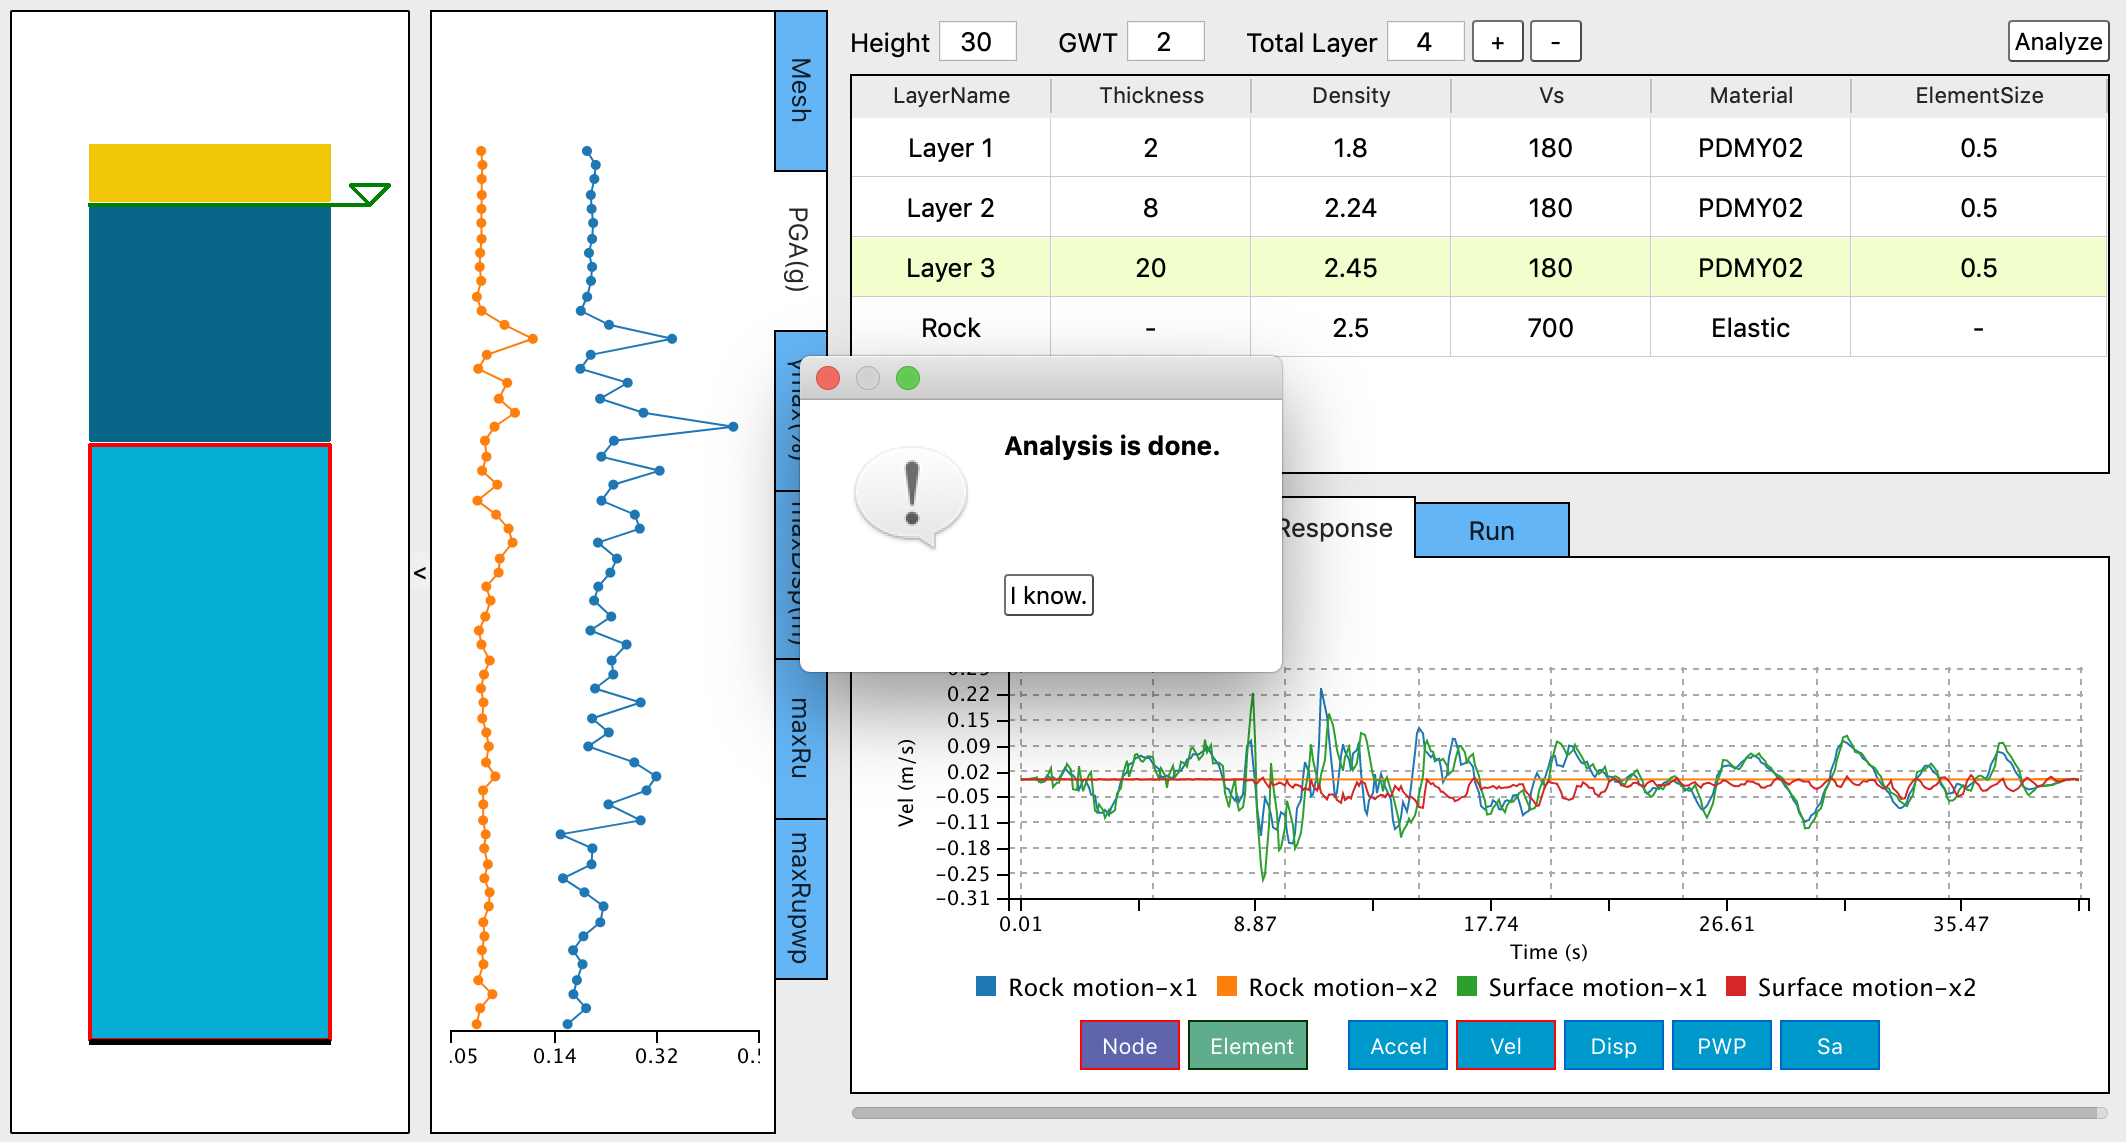
\includegraphics[width=0.9\textwidth]
    {installation/figures/done.png} }
  \caption{Analysis is done }
  \label{fig:done}
\end{figure}

Once the simulation is done, the "Response" tab and the "PGA(g)" profile plot will be displayed.
At the same time, 
a pop up window showing "The analysis is done." will show up.
And when you click "I know.", the progress bar will disappear.

%===============================================================================


\chapter{Usage}
\label{chap:usage}
This option allows users to determine the event at the base of the 
building by performing an effective free-field site response 
analysis of a soil column. In this panel the user specifies a ground 
motion at the bottom of the column. After the soil layers have been properly 
defined, the motion at the ground surface are given at the end 
of the analysis and that motion will be used in the 
simulation of the building response. 



\begin{figure}[!htbp]
  \centering {
    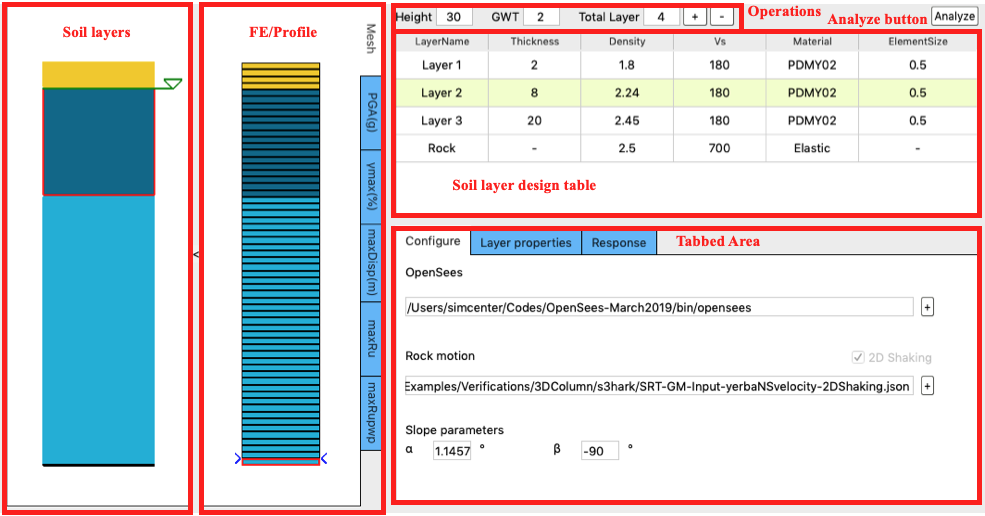
\includegraphics[width=0.8\textwidth]
    {usage/figures/s3hark1.png} }
  \caption{Site Response Analysis Event}
  \label{fig:s3hark1}
\end{figure}

The UI of the Site Response is shown in \Cref{fig:s3hark1}. It is split into the following areas:
\begin{enumerate}
\item Soil Column Graphic: The first graphic on the left of the panel shows a visualization of the soil column.
\item FE Mesh Graphic: The second graphic on the left shows 
the finite element mesh and profile plots. Selecting any of the tabs on the right inside this graphic (i.e, PGA, $\gamma_{max}$, maxDisp, maxRu, maxRuPWP) will show various results
from the simulation at the mesh points.
\item Operations Area: The right side of this area shows some information (e.g., total height and number of soil layers), includes the Ground Water Table (GWT) input field, and plus and minus buttons. 
If the user presses the plus button, a layer is added below the selected layer. If the minus button is pressed the selected layer is removed. The GWT input field allows the user to specify the level of the ground water table.
\item Soil Layer Table: This table is where the user provides the characteristics of the soil layer, such as layer thickness, density, $V_{s30}$, material type, and element size in the finite element mesh.
\item Tabbed Area: This area contains the three tabbed widgets described below.

\begin{figure}[!htbp]
  \centering {
    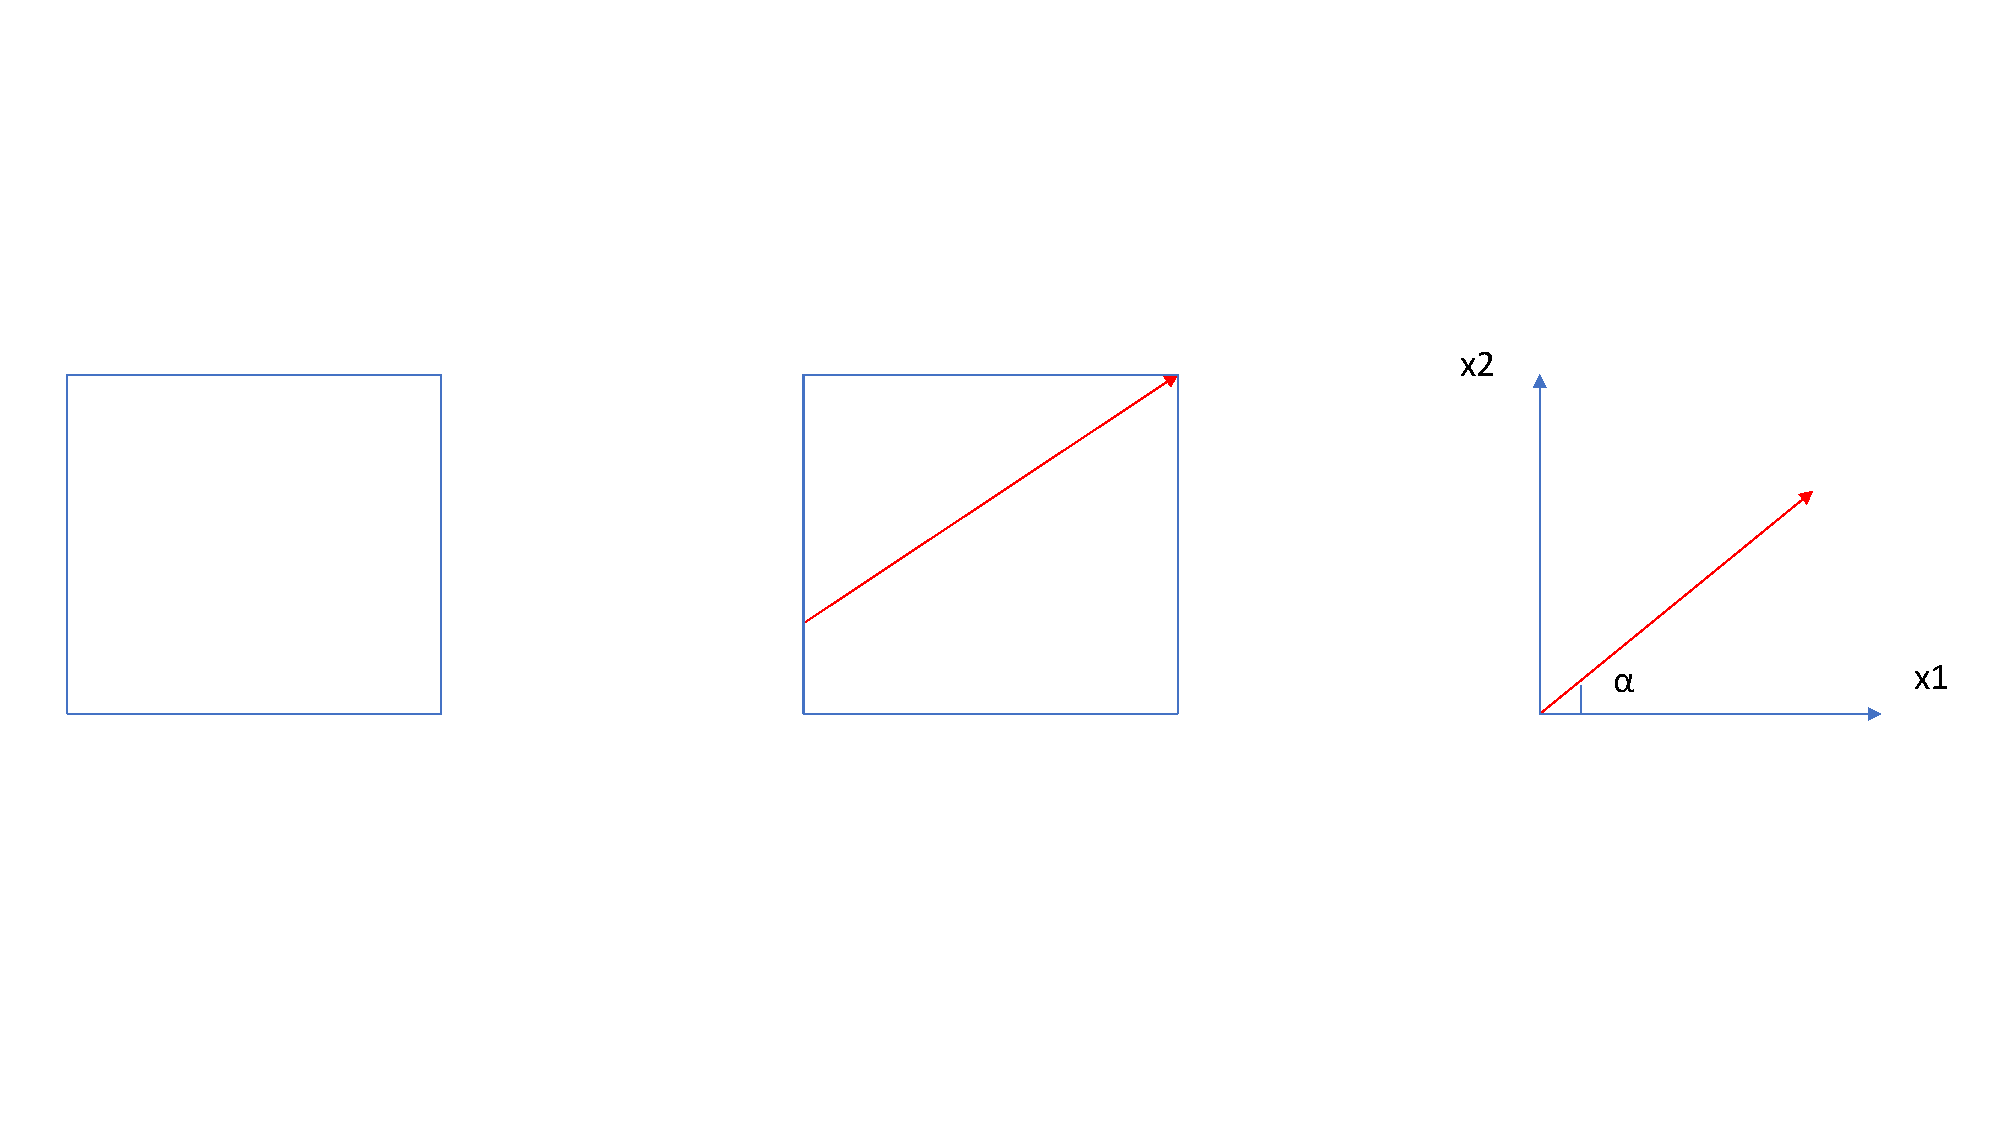
\includegraphics[width=0.8\textwidth]
    {usage/figures/2DSlope.pdf} }
  \caption{Slope definition for 2D Column }
  \label{fig:slope2D}
\end{figure}


\begin{figure}[!htbp]
  \centering {
    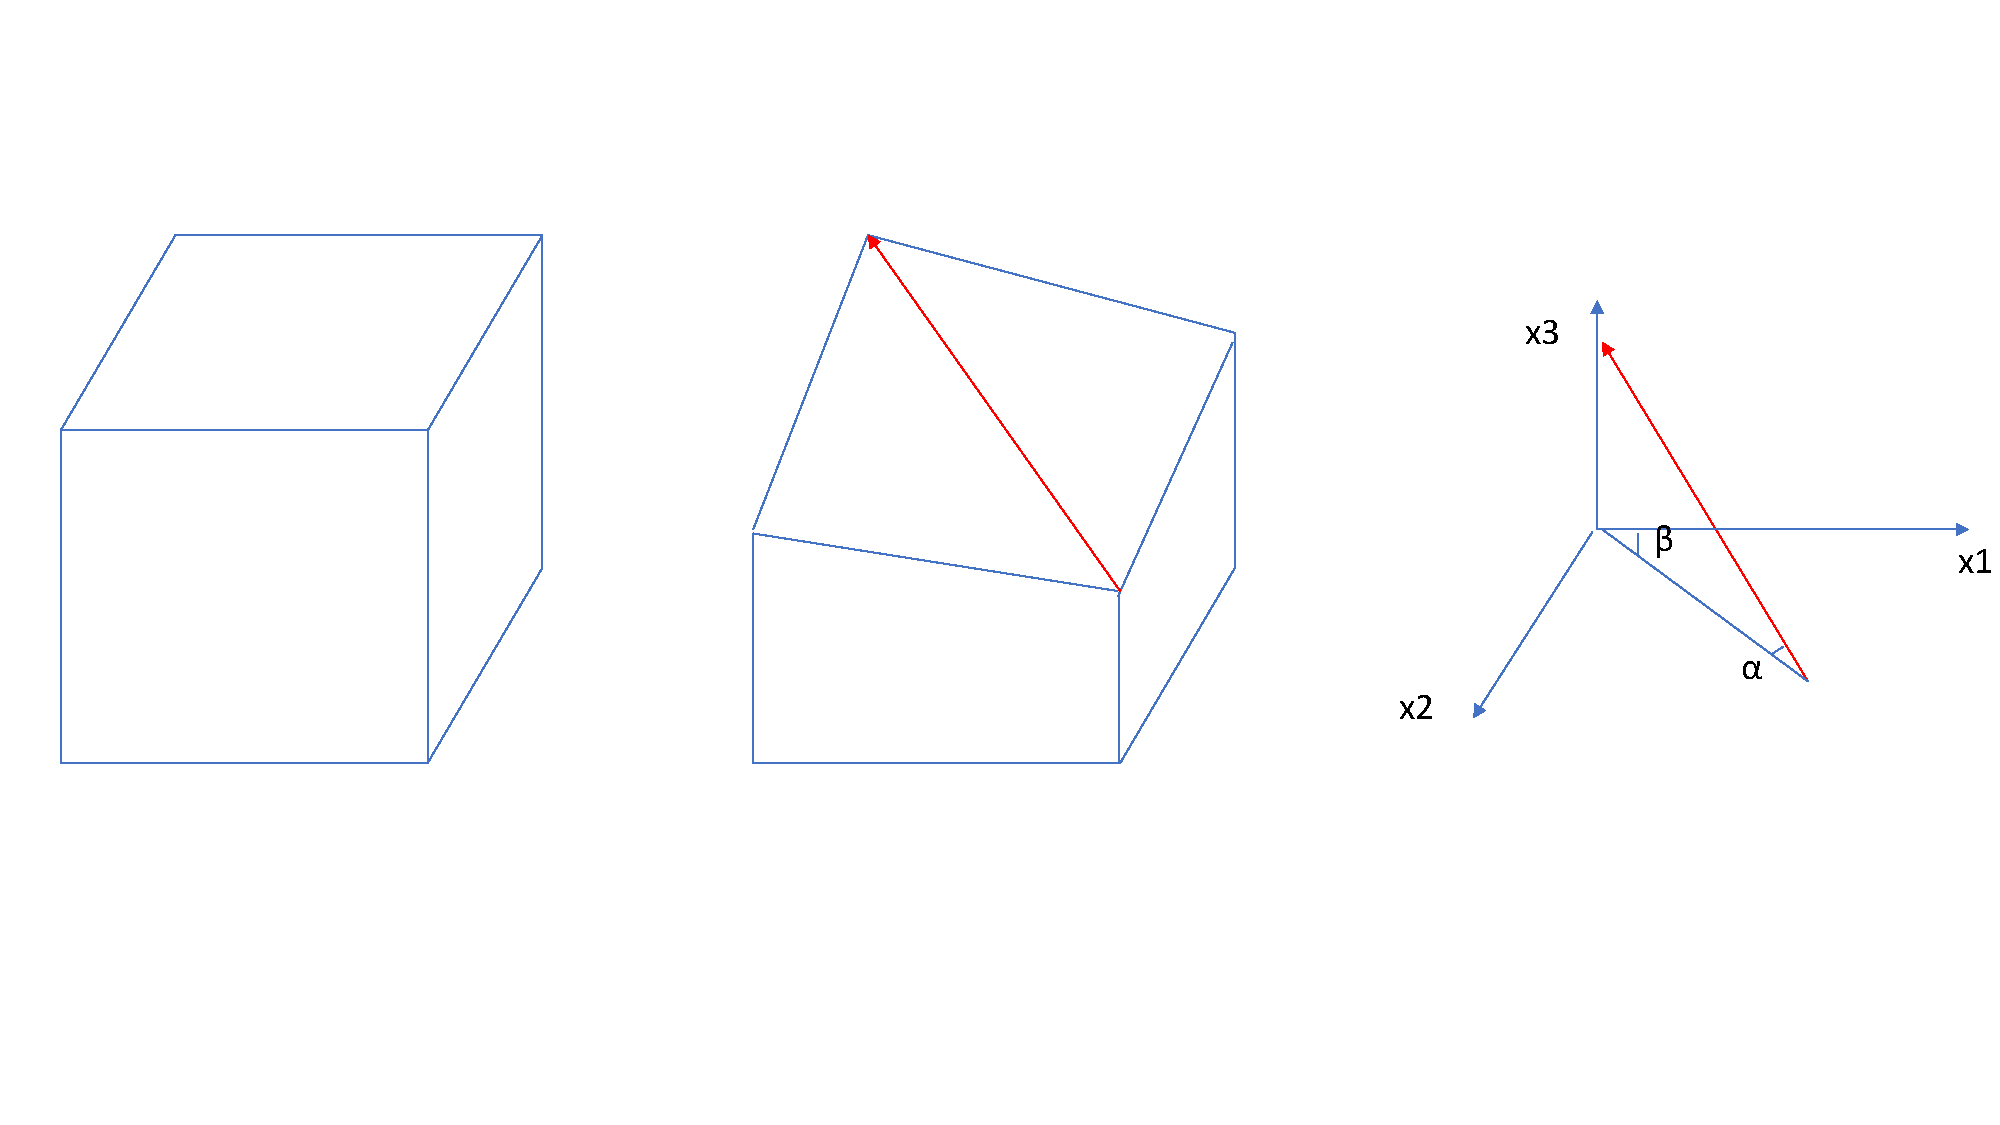
\includegraphics[width=0.8\textwidth]
    {usage/figures/3DSlope.pdf} }
  \caption{Slope definition for 3D Column}
  \label{fig:slope3D}
\end{figure}


\begin{figure}[!htbp]
  \centering {
    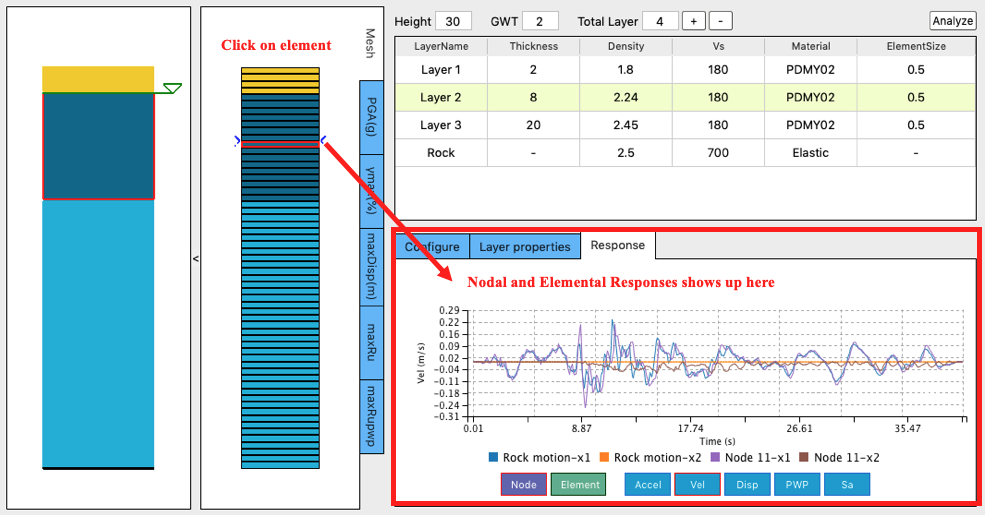
\includegraphics[width=0.8\textwidth]
    {usage/figures/response.png} }
  \caption{Nodal and elemental responses}
  \label{fig:response}
\end{figure}

\begin{enumerate}
  \item Configure Tab: This tab allows the user to specify the path to the OpenSees executable and to a ground motion file that represent the ground shaking at the bedrock. 
  The rock motion file must follow the SimCenter event format. Examples of SimCenter event files are available with the \href{https://github.com/NHERI-SimCenter/EE-UQ/tree/master/example1/event}{source code}.
  \textit{s$^3$hark}  will determine to use 2D column or 3D column based on the ground motion file provided.
  When a ground motion file is selected from the local computer, or the path of the ground motion file is typed in, \textit{s$^3$hark} will figure out if it's a 1D or 2D shaking file. 
  If it's 1D shaking, all elements will be 2D. If it's 2D shaking, all elements will be 3D. The definition of 2D and 3D slope are different. See \Cref{fig:slope2D} and \Cref{fig:slope3D}.
  \item Layer Properties Tab: This tab allows the user to enter additional material properties for the selected soil layer (\Cref{fig:s3hark3}).
  \item Response Tab: Once the site response analysis has been performed, this tab provides information about element and nodal time varying response quantities. See \Cref{fig:response}.
  \item Run Tab: Opens up a window in which by using the up and down arrows on the keyboard the dino will jump up and down. Something to do if the site response analysis is taking too long, which it may if many soil layers are used.
\end{enumerate}

\item Analyze Button: This button shall be used to run the simulation locally. A progress bar will show the status of the analysis. This allows the user to review the ground motion predicted at the surface.
\end{enumerate}

\begin{figure}[!htbp]
  \centering {
    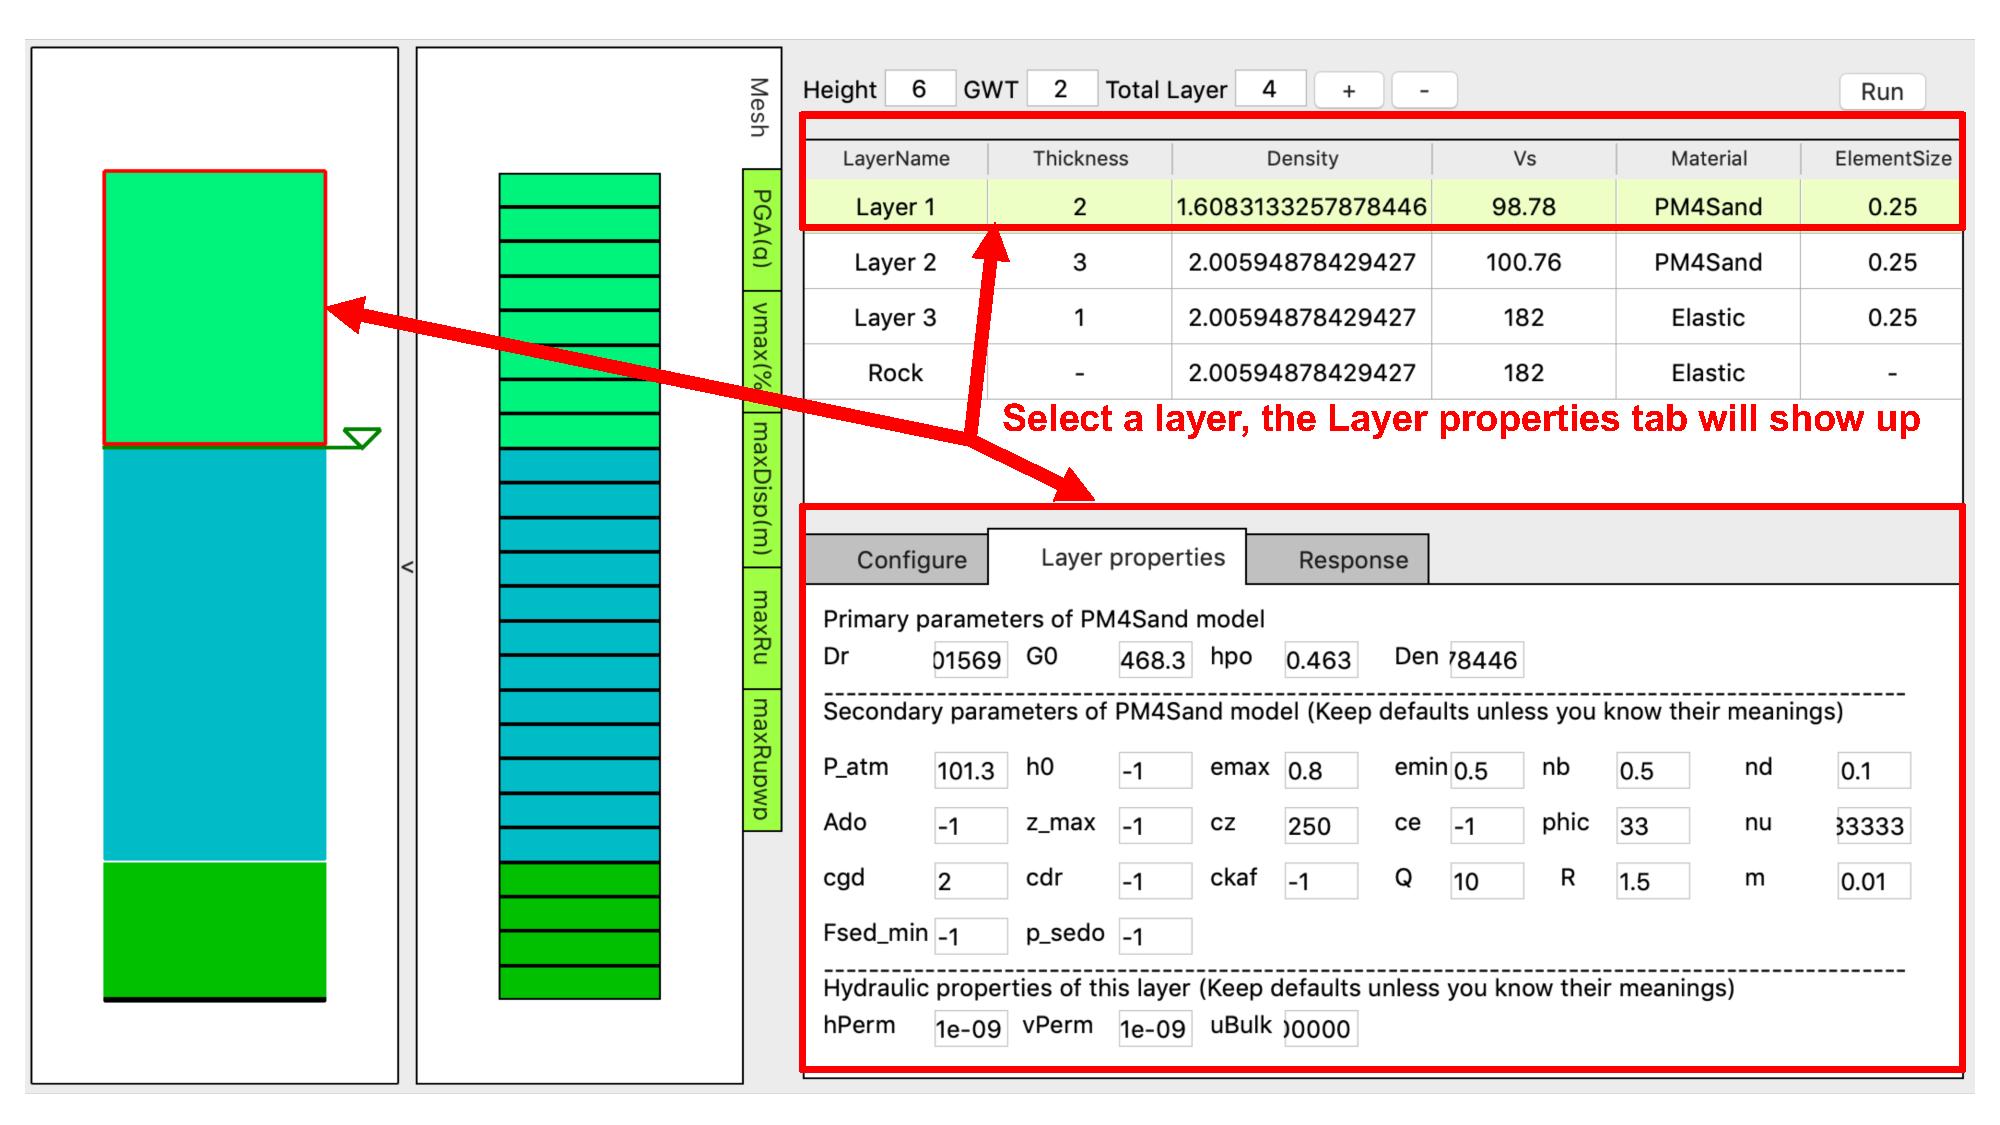
\includegraphics[width=0.8\textwidth]
    {usage/figures/s3hark3.pdf} }
  \caption{Soil Layer Modification in Site Response }
  \label{fig:s3hark3}
\end{figure}

Upon the finish of the finite element analysis, the ground motion at the soil surface (\Cref{fig:s3hark4}) will be stored in EE-UQ's input file.
This computed motion will be applied during the simulation.

\begin{figure}[!htbp]
  \centering {
    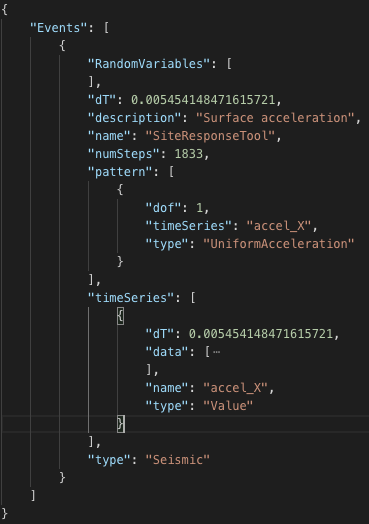
\includegraphics[width=0.4\textwidth]
    {usage/figures/s3hark4.png} }
  \caption{Simulated Motion at the Surface of the Ground}
  \label{fig:s3hark4}
\end{figure}

Random Variables: The current version of the Site Response event type does not support random variables.\\

NOTES: 
\begin{enumerate}
\item Variables are assumed to have m, kPa, and kN units in the Site Response panel.
\item If the Analyze button is not pressed, no simulation will be performed. If no simulation is performed there will be no ground motions provided to the building.
\end{enumerate}



%Select a soil layer by clicking on the design table or by clicking on the graphic soil column.
%When a layer is selected, it will be highlighted in both the design table and the graphic. 
%In the design table, it is highlighted by changing the background color to light green. 


%Given that the properties of the soil layers and the earthquake events are known,
 %\texttt{\getsoftwarename{}} convert provide multiple nonlinear material models for simulating the soil behavior under earthquake loading.


\chapter{Theory and Implementation}
\label{chap:theory}
\texttt{\getsoftwarename{}} is a research application used for performing site-specific analysis of soil in  response to earthquakes. \\


The application focuses on simulating wave propagation along soil depth considering liquefaction 
 using finite element method. There are multiple  advanced constitutive  models implemented: 
PressureDependMultiYield, PressureDependMultiYield02, PressureIndependendMultiYield,
Manzari Dafalias, PM4Sand, PM4Silt, J2CyclicBoundingSurface, ElasticIsotropic.\\

PressureDependMultiYield and PressureDependMultiYield02 materials are elastic-plastic material for simulating the essential response characteristics of pressure sensitive soil materials under general loading conditions. Such characteristics include dilatancy (shear-induced volume contraction or dilation) and non-flow liquefaction (cyclic mobility), typically exhibited in sands or silts during monotonic or cyclic loading.\\



 PressureIndependMultiYield material is an elastic-plastic material in which plasticity exhibits only in the deviatoric stress-strain response. The volumetric stress-strain response is linear-elastic and is independent of the deviatoric response. This material is implemented to simulate monotonic or cyclic response of materials whose shear behavior is insensitive to the confinement change. Such materials include, for example, organic soils or clay under fast (undrained) loading conditions.\\

Manzari Dafalias (\cite{dafalias2004simple}) is a stress-ratio controlled, critical state compatible, sand plasticity model.
A fabric-dilatancy related quantity, scalar valued in the triaxial and tensor valued in generalized stress space, which is instrumental in modeling macroscopically the effect of fabric changes during the dilatant phase of deformation on the subsequent contractant response upon load increment reversals, and the ensuing realistic simulation of the sand behavior under undrained cyclic loading.  The dependence of the plastic strain rate direction on a modified Lode angle in the multiaxial generalization enables it to produce realistic stress-strain simulations in nontriaxial conditions. A very systematic connection between the simple triaxial and the general multiaxial formulation makes it possible to use correctly the model parameters of the former in the implementation of the latter. \\



The sand plasticity model PM4Sand (version 3) \cite{boulanger2015pm4sand} follows the basic framework of the stress-ratio controlled, critical
state compatible, bounding surface plasticity model for sand presented by  \cite{dafalias2004simple}.
Modifications to the model were developed by \cite{boulanger2015pm4sand} to improve its ability to
approximate the stress-strain responses important to geotechnical earthquake engineering applications;
in essence, the model was calibrated at the equation level to provide for better approximation of the
trends observed across a set of experimentally- and case history-based design correlations. 
The model is shown to provide reasonable approximations of desired behaviors and to be relatively easy to calibrate. \\



PM4Silt (\cite{boulanger2018pm4silt}) is a plasticity model for representing low-plasticity silts and clays in geotechnical earthquake engineering applications .
 The PM4Silt model builds on the framework of the stress-ratio controlled, critical state compatible, bounding surface plasticity PM4Sand model. 
 Modifications to the model were developed and implemented to improve its ability to approximate undrained monotonic and cyclic loading responses of low-plasticity silts and clays, as opposed to those for purely nonplastic silts or sands. Emphasis was given to obtaining reasonable approximations of undrained monotonic shear strengths, undrained cyclic shear strengths, and shear modulus reduction and hysteretic damping responses across a range of initial static shear stress and overburden stress conditions. The model does not include a cap, and therefore is not suited for simulating consolidation settlements or strength evolution with consolidation stress history. The model is cast in terms of the state parameter relative to a linear critical state line in void ratio versus logarithm of mean effective stress. The primary input parameters are the undrained shear strength ratio (or undrained shear strength), the shear modulus coefficient, the contraction rate parameter, and an optional post-strong-shaking shear strength reduction factor. \\
 
 J2CyclicBoundingSurface (\cite{borja1994multiaxial}) is a 
  total stress‐based bounding surface plasticity model for clays developed to accommodate multiaxial stress reversals. 
  The model is constructed based on the idea of a vanishing elastic region undergoing pure translation inside a bounding surface, and an interpolation function for hardening modulus which varies with stress distance of the elastic region from the unloading point. 
  Central to the development of the model are the general criteria for loading and unloading, 
  which are phrased based upon the simple argument that with continued loading the hardening modulus should decrease monotonically with deformation. 
  Combined with numerical integration of the elastoplastic constitutive equations in a form suitable for a robust computer implementation, 
  the model is applied to cohesive soils undergoing undrained stress reversals and cyclic loading. 
  With a suitable choice of the interpolation function for the hardening modulus,
   it is shown that existing one‐dimensional nonlinear laws for soils can be replicated, 
   such as the hyperbolic, exponential, the Davidenkov, and even the Ramberg‐Osgood models. 
   Specifically, the appropriateness of the exponential hardening function for cohesive soils is investigated and its parameters determined for some clays and silts for use in dynamic soil‐structure interaction modeling.\\




\chapter{Source Code}
\label{chap:SourceCode}
This source code for the tool is released under the 2-clause BSD
License, commonly called the FreeBSD license.  It is available for
download from the
tool's \href{https://github.com/NHERI-SimCenter/s3hark}{GitHub
repository}

\chapter{User Training}
\label{chap:training}
User Training consists of an online video available from the tool
webpage that demonstrates tool use. The tool will be presented in user
workshops hosted by the SimCenter.



\chapter{Verification and Validation by Examples}
\label{chap:vnv}
A 2D free field effective stress analysis is performed by s$^3$hark
and demonstrated here.  The results are verified against FLAC and
Plaxis.  The soil column being analyzed is 6 meters high sitting on a
rock.  The ground water table is at 2 meters below the soil surface.
In the column, there are a total of three soil layers. Each layer is
meshed by elements with a size of 0.25 meter in height.  Basic
properties of soil layers and the rock are shown
in \autoref{fig:s3harkSoilColumn} and \autoref{fig:s3hark5}.  The
first two layers are modeled by PM4Sand and the third layer is modeled
by elastic isotropic material.  (The implementation work of
PM4Sand \cite{boulanger2015pm4sand} is done in University of
Washington by Long Chen and Pedro Arduino.  Chaofeng Wang at UC,
Berkeley contributed to the code optimization for speed improvement. )
The rock layer will be simplified to a \cite{Lysmer:1969} dashpot,
which accounts for the finite rigidity of the underlying elastic
medium.  The parameters of the dashpot are calculated solely based on
rock layer's density and V$_{s30}$.


\begin{figure}[!htbp]
  \centering {
    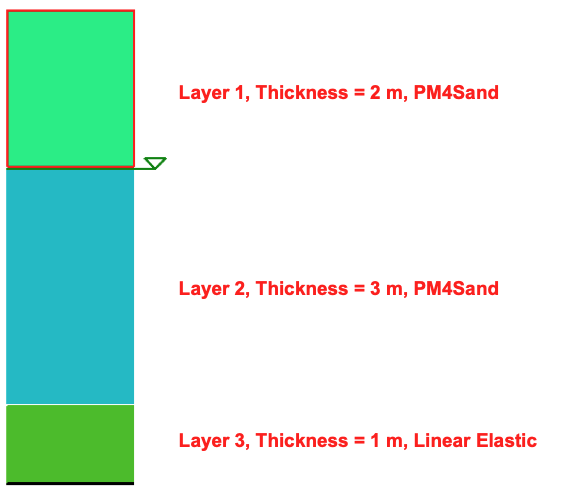
\includegraphics[width=0.5\textwidth]
    {ver_and_val/figures/s3harkSoilColumn.png} }
  \caption{Soil layers }
  \label{fig:s3harkSoilColumn}
\end{figure}


\begin{figure}[!htbp]
  \centering {
    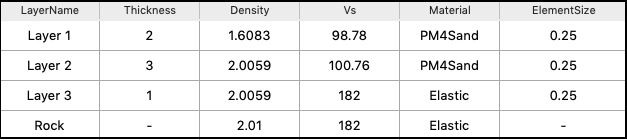
\includegraphics[width=0.5\textwidth]
    {ver_and_val/figures/s3hark5.png} }
  \caption{Soil layers }
  \label{fig:s3hark5}
\end{figure}


The detailed properties of the material in each soil layer are shown in \autoref{fig:s3hark6}.

\begin{figure}[!htbp]
  \centering 
  \subfloat[Layer 1]{
    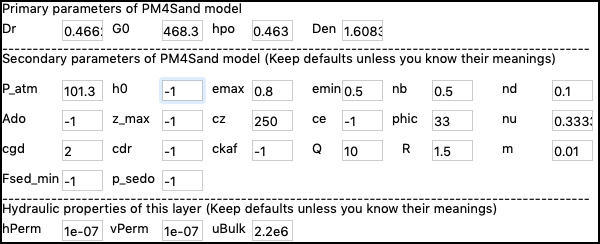
\includegraphics[width=0.4\textwidth]
    {ver_and_val/figures/layer1.png}}
  \subfloat[Layer 2]{
    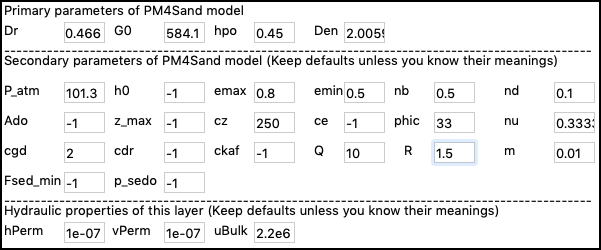
\includegraphics[width=0.39\textwidth]
    {ver_and_val/figures/layer2.png}}
    
    \subfloat[Layer 3]{
    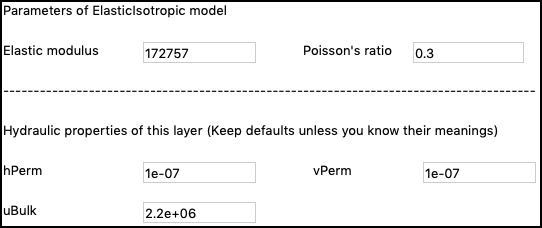
\includegraphics[width=0.4\textwidth]
    {ver_and_val/figures/layer3.png}}
  \caption{Detail soil properties and material model parameters}
  \label{fig:s3hark6}
\end{figure}

For the verification and validation purposes, s$^3$hark's results are compared with FLAC an PLAXIS, as shown in \autoref{fig:s3hark7}. 
All three programs generally produce very similar response with
different levels of differences shown in PHA, maximum shear strain, CSR, maximum pore pressure ratio. 
The differences come from multiple sources, such as numerical discretization methods, solvers, etc.
For example, FLAC tends to produce higher dilation pulses in liquefied layer. 
This is possibly due to a combination of different reasons, e.g.,
interpolation of data from integration points at different
locations, numerical methods for integration, formulations for
solid fluid coupling, etc.
(Chaofeng Wang at UC, Berkeley, Long Chen and Andrew Makdisi at University of Washington,  
Gregor Vilhar at PLAXIS, BV contributed to the verification of PM4Sand in s$^3$hark. )

\begin{figure}[!htbp]
  \centering {
    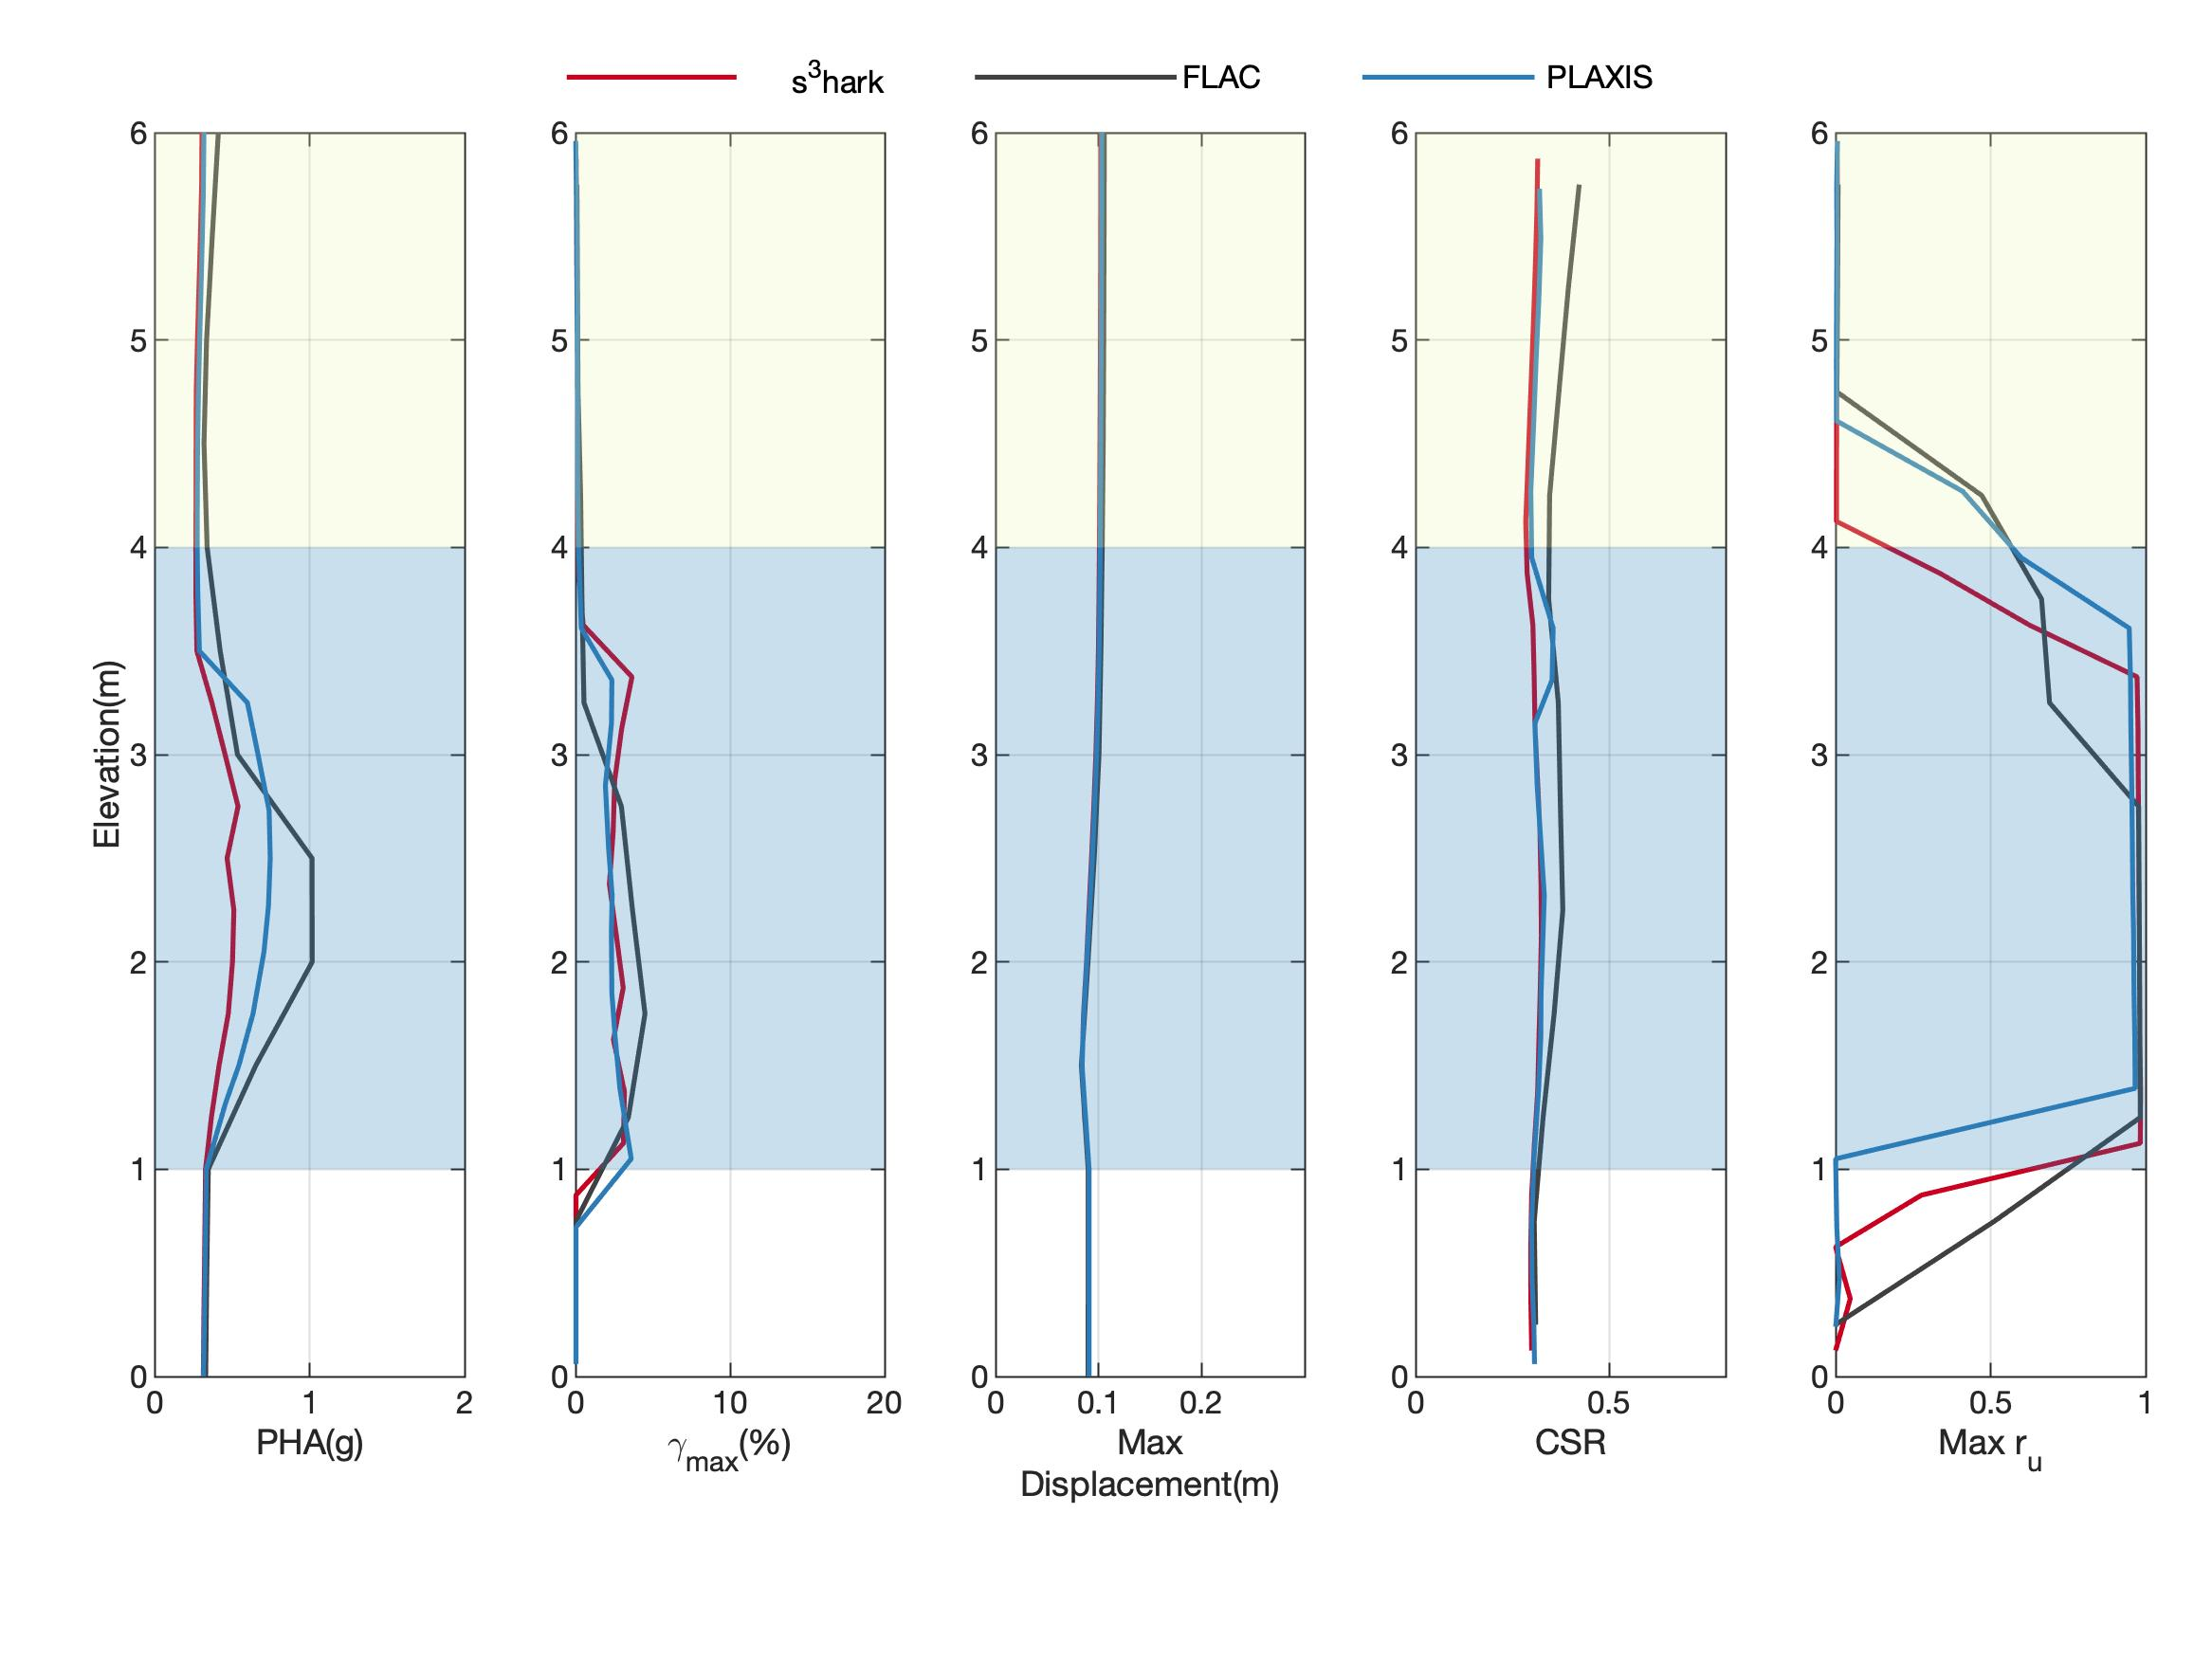
\includegraphics[width=0.7\textwidth]
    {ver_and_val/figures/N10T3_RSN766_ProfileCompare.jpg} }
  \caption{Soil layers }
  \label{fig:s3hark7}
\end{figure}




\nocite{*}

% \appendix
% \chapter{More Monticello Candidates}

\pagestyle{plain}
{
  \renewcommand{\thispagestyle}[1]{}	
  \printbibliography           
}

\end{document}
